\documentclass[lettersize,journal]{IEEEtran}
\usepackage{amsmath,amsfonts}
\usepackage{algorithmic}
\usepackage{algorithm}
\usepackage{array}
\usepackage[caption=false,font=normalsize,labelfont=sf,textfont=sf]{subfig}
\usepackage{textcomp}
\usepackage{stfloats}
\usepackage{url}
\usepackage{verbatim}
\usepackage{graphicx}
\usepackage{cite}
\hyphenation{op-tical net-works semi-conduc-tor IEEE-Xplore}

\begin{document}

\title{OUXT Polaris: Autonomous Navigation System for the 2022 Maritime RobotX Challenge}
\author{
    Kenta Okamoto,Kyoto Institute of Tech., m2623106@edu.kit.ac.jp \\ \and
    Akihisa Nagata, Kansai Univ. , k065604@kansai-u.ac.jp \\ \and
    Masato Kobayashi, Kobe Univ. , 171w951w@gsuite.kobe-u.ac.jp \\ \and
    Shunya Tanaka, , syun111@gmail.com \\ \and
    Masaya Kataoka, TEIR IV inc . , ms.kataoka@gmail.com,
}

% The paper headers
\markboth{IEEE TRANSACTIONS ON XXXXX,~Vol.~xx, No.~x, XXX~2022}%
{Shell \MakeLowercase{\textit{et al.}}: A Sample Article Using IEEEtran.cls for IEEE Journals}

% \IEEEpubid{0000-0000/00\$00.00~\copyright~2021 IEEE}
% Remember, if you use this you must call \IEEEpubidadjcol in the second
% column for its text to clear the IEEEpubid mark.

\maketitle

\begin{abstract}
OUXT-Polaris has been developing an autonomous navigation system by participating in the 
Maritime RobotX Challenge 2014, 2016, and 2018. 
In this paper, we describe the improvement of the previous vessel system. 
We also indicate the advantage of the improved design.
Moreover, we describe the developing method for Covid-19 and the 
feature components for the next RobotX Challenge.
\end{abstract}

\begin{IEEEkeywords}
Maritime systems, Robotics, Unmanned surface vehicle
\end{IEEEkeywords}

\section{Introduction}
First of all, we are motivated to develop a big field robot in a large area such as the ocean.
In recent years, the aging and shrinking population, as well as a shortage of workers,
has led to an increase in demand for the automation of cars, robots, and other equipment.
Among these, automated driving is being developed with particular emphasis.
Moving the autonomous vehicle or robot outside has a very severe problem.
They need to hedge unknown obstacles and go to the target position.
The environment such as weather, temperature, or underwater around robots causes sensor and hardware problems.
There are each challenging problems and They are also interesting for us, and there are different problems between land and ocean.
On the land, the navigation or the estimation of the self-position is solved by the point cloud map and the odmetry,
while on the ocean, the point cloud and the odmetry is not obtained enough. So the robots need to estimate the self-position using GPS and IMU sensors.
Moreover, on the land, the position of the target objects and obstacles is obtained from Lidar data. On the other hand in the sea,
waves disturbe to get the target positions. In that case, the robots have to fusion multiple data such as cameras and Lidars.
In this competition, we have a chance to develop a system to get over the wild environment 
for the robots on the ocean. Therefore, we are participating in the Maritime RobotX Challenge.

\section{Overview of vessel system}
First, we describe the architecture of the navigation system. As you can see \ref{fig:arch_nav},
the position and the velocity of WAM-V are estimated using the Extended Kalman Filter from the data of the GNSS and IMU sensors.
The obstacles and task objects are recognized from lidar and camera data. Based on the self-position and the task objects, 
WAM-V decides where to go and what to do next. After getting the target position, the path is created by the path planner, and the target velocity that WAM-V can trace the way is
calculated. 
Finally, in the servo and thruster controllers, the servo motor direction and the thruster revolution to achieve the target velocity are calculated based on the vessel motion model.

\begin{figure}[h]
  \begin{center}
    \scalebox{0.24}{
      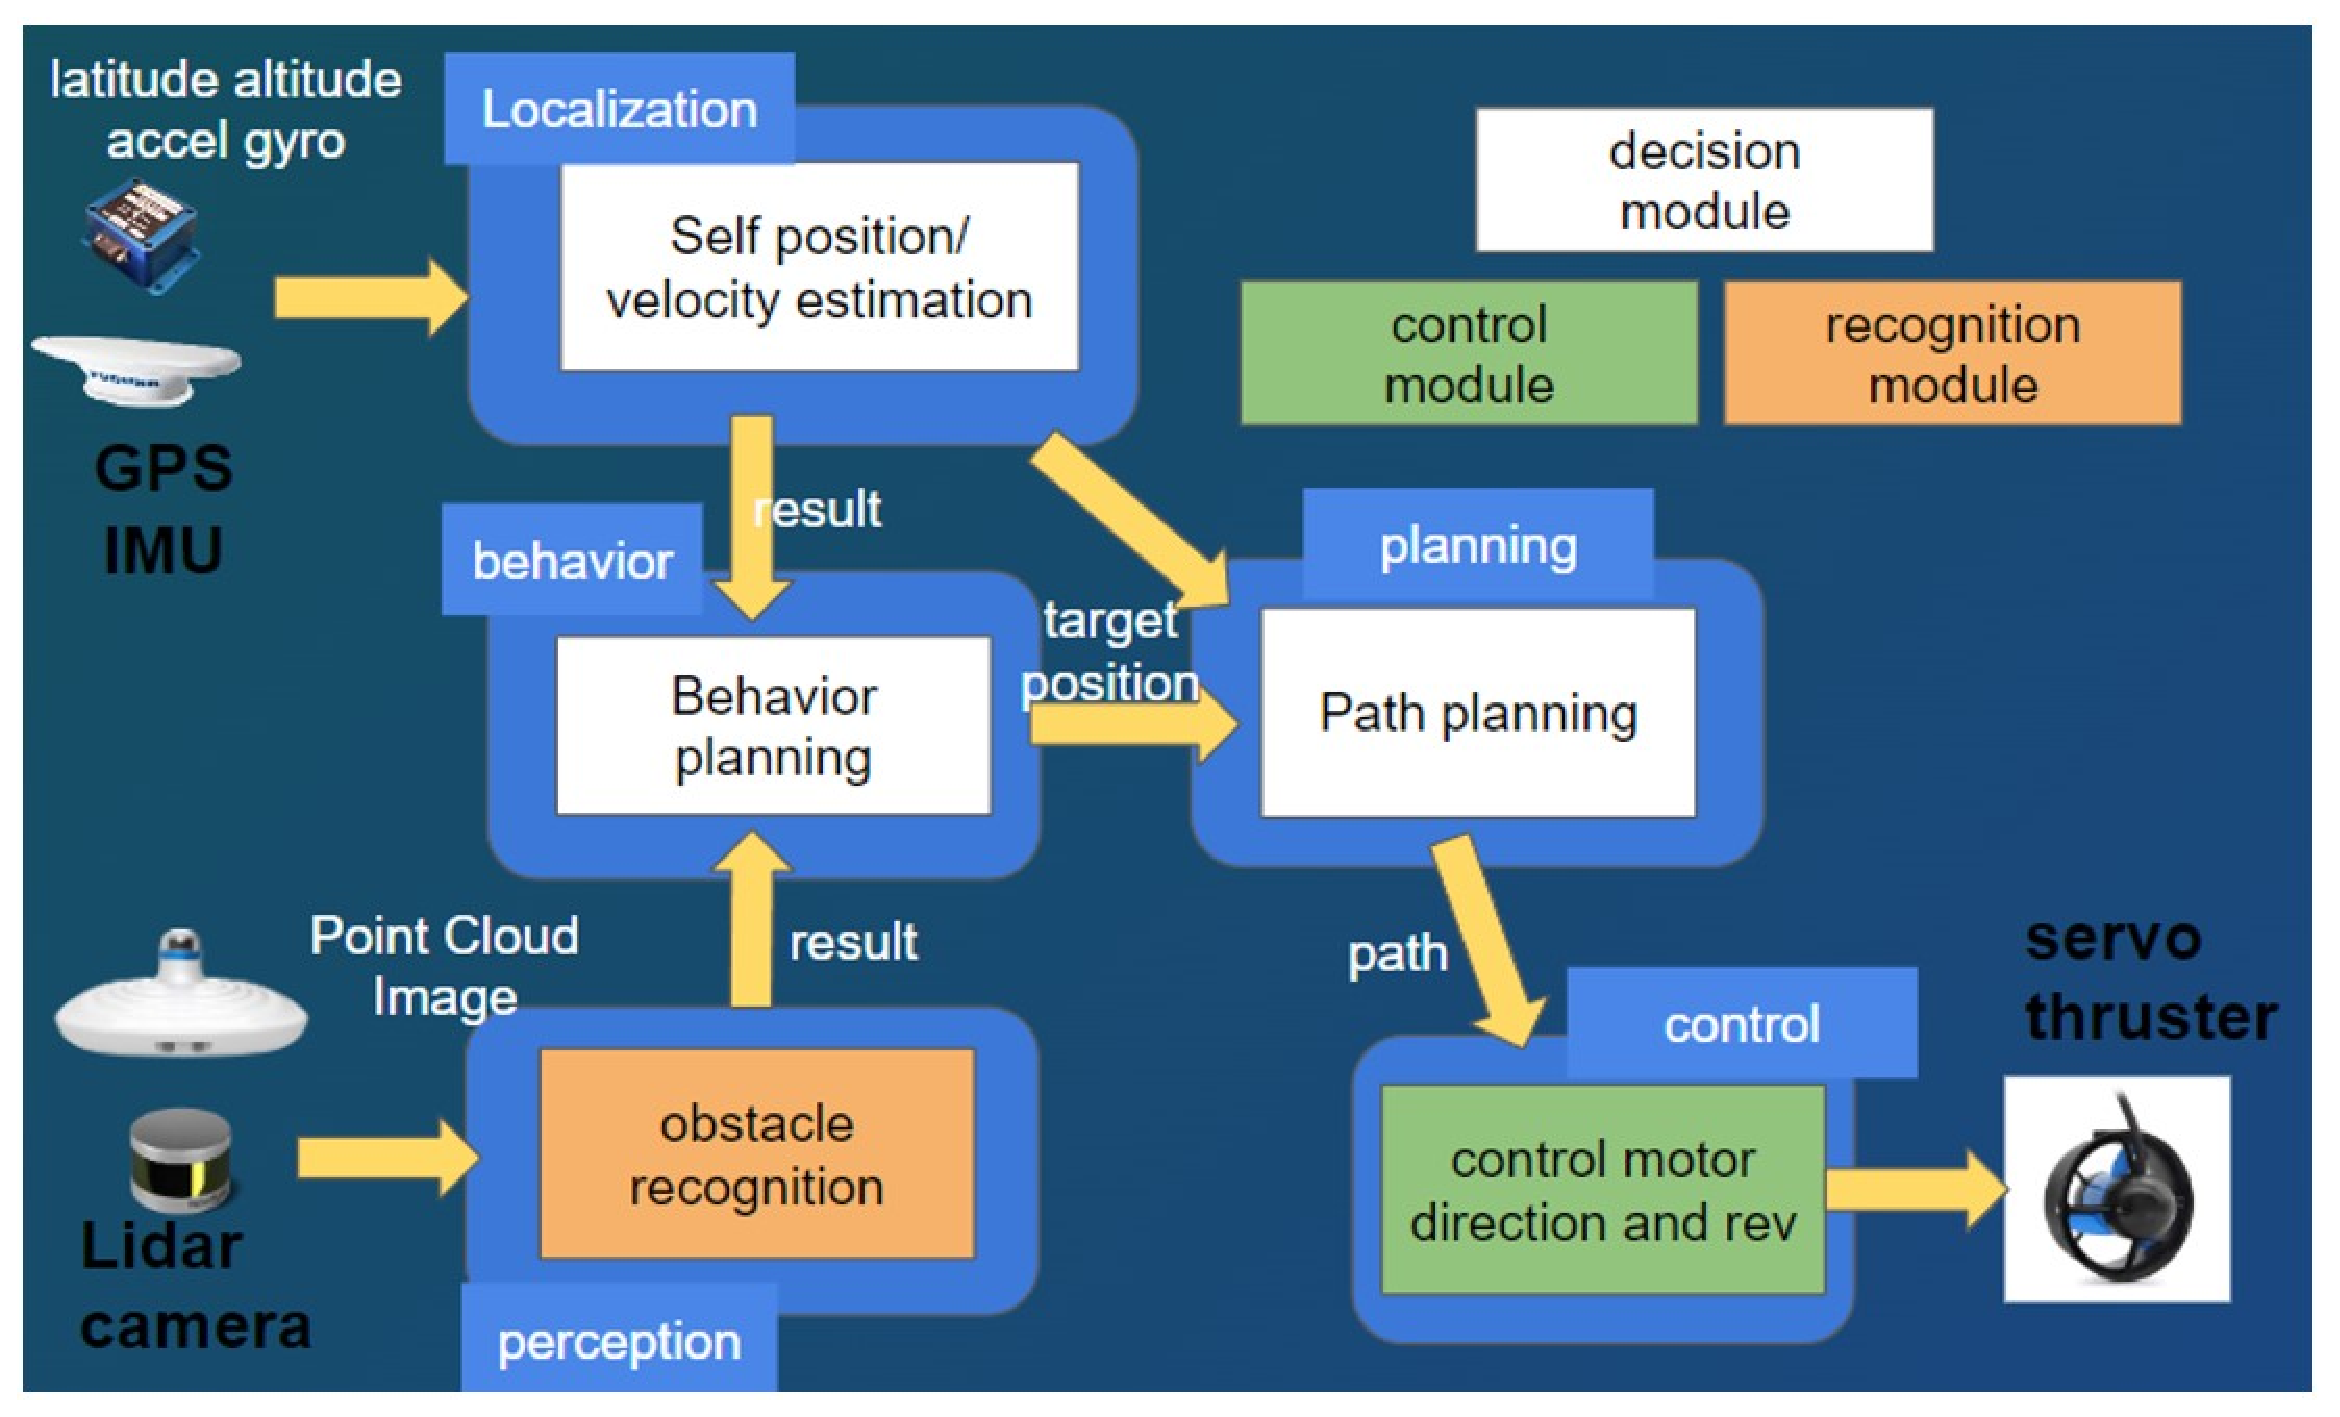
\includegraphics{figure/arch_nav.eps}
    }
  \end{center}
  \caption{the archtecture of navigation system}
  \label{fig:arch_nav}
\end{figure}




\section{Conclusion}
XXXXXX
% \section*{Acknowledgments}
\begin{thebibliography}{1}
\bibliographystyle{IEEEtran}

  \bibitem{YOLOX}
  Ge, Zheng, et al. "Yolox: Exceeding yolo series in 2021." arXiv preprint arXiv:2107.08430 (2021).

  \bibitem{RobotX2018_video}
  \url{https://www.youtube.com/watch?v=MqDBxzS4uy4}

\end{thebibliography}

\vfill

\end{document}